
\documentclass[border=10pt, 12pt]{standalone}
\usepackage[svgnames]{xcolor}
\usepackage{amsmath}
\usepackage{pgfplots}
\pgfplotsset{compat=newest}
\usepackage[sfdefault]{FiraSans}
\usepackage{FiraMono}
\renewcommand*\familydefault{\sfdefault}
\begin{document}
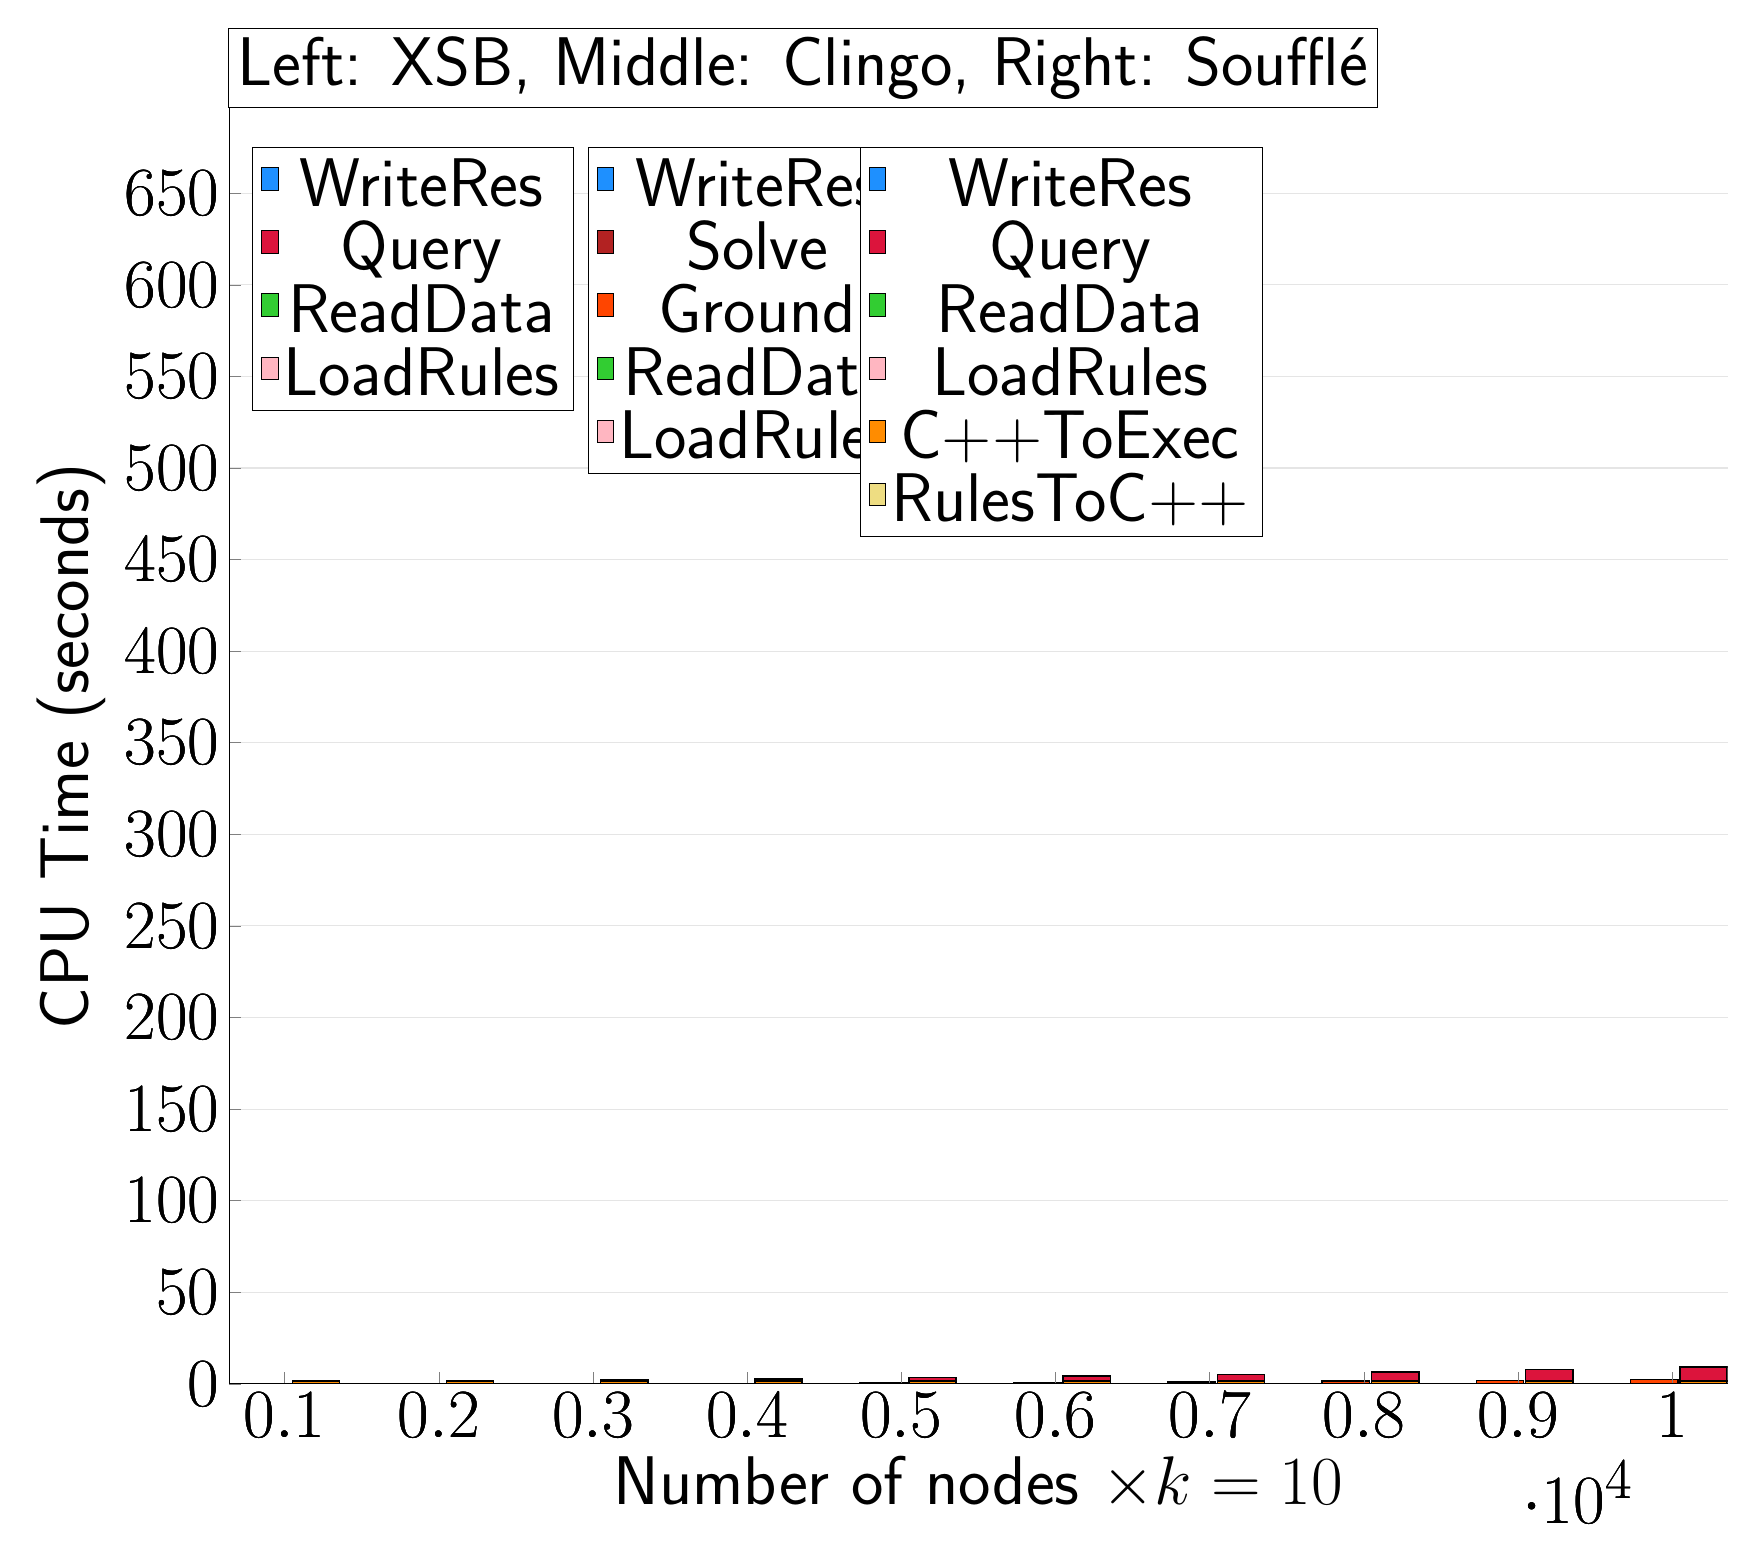
\begin{tikzpicture}
                        \begin{axis}[bar shift=-24.3pt, 
   ybar stacked,
   width=1.7\textwidth,
   bar width=0.6cm,
   ymajorgrids, tick align=inside,
   major grid style={draw=gray!20},
   xtick=data,
   ymin=0, ymax=696.3414,
   axis x line*=bottom,
   axis y line*=left,
   enlarge x limits=0.04,
   legend style={
       at={(0.23, 0.97)},
       anchor=north east,
       legend columns=1,
       font=\Huge,
   },
   ylabel={CPU Time (seconds)},
   xlabel={Number of nodes $\times k=10$},
   label style={font=\Huge},
   tick label style={font=\Huge},
]
\addlegendimage{fill=DodgerBlue, draw=black, line width=0.2pt}
\addlegendentry{WriteRes}
\addlegendimage{fill=Crimson, draw=black, line width=0.2pt}
\addlegendentry{Query}
\addlegendimage{fill=LimeGreen, draw=black, line width=0.2pt}
\addlegendentry{ReadData}
\addlegendimage{fill=LightPink, draw=black, line width=0.2pt}
\addlegendentry{LoadRules}
\addplot +[fill=LightPink, draw=black, line width=0.55pt] coordinates {
(1000, 0.0005632000000000002)
(2000, 0.0005558000000000006)
(3000, 0.0005533999999999996)
(4000, 0.0005529999999999995)
(5000, 0.0005520000000000001)
(6000, 0.0005576000000000003)
(7000, 0.0005548)
(8000, 0.0005496000000000001)
(9000, 0.0005540000000000005)
(10000, 0.0005521999999999999)
};
\addplot +[fill=LimeGreen, draw=black, line width=0.55pt] coordinates {
(1000, 0.0009075999999999994)
(2000, 0.0017318)
(3000, 0.0025930000000000003)
(4000, 0.0033894)
(5000, 0.004226)
(6000, 0.0050638)
(7000, 0.0058282)
(8000, 0.0066858)
(9000, 0.007536800000000001)
(10000, 0.0083354)
};
\addplot +[fill=Crimson, draw=black, line width=0.55pt] coordinates {
(1000, 0.0001846000000000006)
(2000, 0.0006749999999999992)
(3000, 0.001454)
(4000, 0.0025676)
(5000, 0.0039726)
(6000, 0.0057174)
(7000, 0.0078011999999999995)
(8000, 0.0100998)
(9000, 0.0127444)
(10000, 0.0157514)
};
\addplot +[fill=DodgerBlue, draw=black, line width=0.55pt] coordinates {
(1000, 9.41999999999996e-05)
(2000, 0.00012120000000000124)
(3000, 0.00014939999999999997)
(4000, 0.0001763999999999999)
(5000, 0.0001901999999999999)
(6000, 0.00024519999999999994)
(7000, 0.00024799999999999963)
(8000, 0.00032460000000000025)
(9000, 0.00044620000000000006)
(10000, 0.0003394000000000001)
};
\end{axis}

\begin{axis}[bar shift=-6.5pt, 
   ybar stacked,
   width=1.7\textwidth,
   bar width=0.6cm,
   ymajorgrids, tick align=inside,
   major grid style={draw=none},
   xtick=data,
   ymin=0, ymax=696.3414,
   axis x line*=none,
   axis y line*=none,
   enlarge x limits=0.04,
   legend style={
       at={(0.454, 0.97)},
       anchor=north east,
       legend columns=1,
       font=\Huge,
   },
   label style={font=\Huge},
   tick label style={font=\Huge},
]
\addlegendimage{fill=DodgerBlue, draw=black, line width=0.2pt}
\addlegendentry{WriteRes}
\addlegendimage{fill=FireBrick, draw=black, line width=0.2pt}
\addlegendentry{Solve}
\addlegendimage{fill=OrangeRed, draw=black, line width=0.2pt}
\addlegendentry{Ground}
\addlegendimage{fill=LimeGreen, draw=black, line width=0.2pt}
\addlegendentry{ReadData}
\addlegendimage{fill=LightPink, draw=black, line width=0.2pt}
\addlegendentry{LoadRules}
\addplot +[fill=LightPink, draw=black, line width=0.55pt] coordinates {
(1000, 0.0)
(2000, 0.0)
(3000, 0.0)
(4000, 0.0)
(5000, 0.0)
(6000, 0.0)
(7000, 0.0)
(8000, 0.0)
(9000, 0.0)
(10000, 0.0)
};
\addplot +[fill=LimeGreen, draw=black, line width=0.55pt] coordinates {
(1000, 0.0)
(2000, 0.0)
(3000, 0.008000000000000007)
(4000, 0.010000000000000009)
(5000, 0.010000000000000009)
(6000, 0.010000000000000009)
(7000, 0.010000000000000009)
(8000, 0.018000000000000016)
(9000, 0.020000000000000018)
(10000, 0.020000000000000018)
};
\addplot +[fill=OrangeRed, draw=black, line width=0.55pt] coordinates {
(1000, 0.020000000000000018)
(2000, 0.07)
(3000, 0.16200000000000003)
(4000, 0.29200000000000004)
(5000, 0.5)
(6000, 0.756)
(7000, 1.046)
(8000, 1.378)
(9000, 1.86)
(10000, 2.2540000000000004)
};
\addplot +[fill=FireBrick, draw=black, line width=0.55pt] coordinates {
(1000, 0.0)
(2000, 0.0040000000000000036)
(3000, 0.0)
(4000, 0.008000000000000007)
(5000, 0.010000000000000009)
(6000, 0.008000000000000007)
(7000, 0.014000000000000012)
(8000, 0.018000000000000016)
(9000, 0.02400000000000002)
(10000, 0.028000000000000025)
};
\addplot +[fill=DodgerBlue, draw=black, line width=0.55pt] coordinates {
(1000, 0.0)
(2000, -0.0040000000000000036)
(3000, 0.0)
(4000, -0.008000000000000007)
(5000, -0.010000000000000009)
(6000, -0.0040000000000000036)
(7000, -0.014000000000000012)
(8000, -0.016000000000000014)
(9000, -0.022000000000000065)
(10000, -0.028000000000000025)
};
\end{axis}

\begin{axis}[bar shift=11.3pt, 
   ybar stacked,
   width=1.7\textwidth,
   bar width=0.6cm,
   ymajorgrids, tick align=inside,
   major grid style={draw=none},
   xtick=data,
   ymin=0, ymax=696.3414,
   axis x line*=none,
   axis y line*=none,
   enlarge x limits=0.04,
   legend style={
       at={(0.69, 0.97)},
       anchor=north east,
       legend columns=1,
       font=\Huge,
   },
   label style={font=\Huge},
   tick label style={font=\Huge},
]
\addlegendimage{fill=DodgerBlue, draw=black, line width=0.2pt}
\addlegendentry{WriteRes}
\addlegendimage{fill=Crimson, draw=black, line width=0.2pt}
\addlegendentry{Query}
\addlegendimage{fill=LimeGreen, draw=black, line width=0.2pt}
\addlegendentry{ReadData}
\addlegendimage{fill=LightPink, draw=black, line width=0.2pt}
\addlegendentry{LoadRules}
\addlegendimage{fill=DarkOrange, draw=black, line width=0.2pt}
\addlegendentry{C++ToExec}
\addlegendimage{fill=LightGoldenrod, draw=black, line width=0.2pt}
\addlegendentry{RulesToC++}
\addplot +[fill=LightGoldenrod, draw=black, line width=0.55pt] coordinates {
(1000, 0.006000000000000001)
(2000, 0.006000000000000001)
(3000, 0.004000000000000001)
(4000, 0.008000000000000002)
(5000, 0.008000000000000002)
(6000, 0.008000000000000002)
(7000, 0.0020000000000000005)
(8000, 0.0020000000000000005)
(9000, 0.006000000000000001)
(10000, 0.004000000000000001)
};
\addplot +[fill=DarkOrange, draw=black, line width=0.55pt] coordinates {
(1000, 1.52)
(2000, 1.5260000000000002)
(3000, 1.5340000000000003)
(4000, 1.5240000000000002)
(5000, 1.5219999999999998)
(6000, 1.53)
(7000, 1.526)
(8000, 1.538)
(9000, 1.528)
(10000, 1.536)
};
\addplot +[fill=LightPink, draw=black, line width=0.55pt] coordinates {
(1000, 0.00014240000000000002)
(2000, 0.00014560000000000002)
(3000, 0.000149)
(4000, 0.0001514)
(5000, 0.0001438)
(6000, 0.00014720000000000003)
(7000, 0.0001404)
(8000, 0.0001464)
(9000, 0.00013879999999999999)
(10000, 0.00014580000000000002)
};
\addplot +[fill=LimeGreen, draw=black, line width=0.55pt] coordinates {
(1000, 0.0040566)
(2000, 0.0069688)
(3000, 0.0100524)
(4000, 0.011537400000000001)
(5000, 0.0143618)
(6000, 0.0157858)
(7000, 0.0180972)
(8000, 0.019448399999999998)
(9000, 0.020607999999999998)
(10000, 0.0243608)
};
\addplot +[fill=Crimson, draw=black, line width=0.55pt] coordinates {
(1000, 0.0790184)
(2000, 0.2781424)
(3000, 0.6340532)
(4000, 1.150434)
(5000, 1.82407)
(6000, 2.653614)
(7000, 3.6612540000000005)
(8000, 4.825256)
(9000, 6.17586)
(10000, 7.689628000000001)
};
\addplot +[fill=DodgerBlue, draw=black, line width=0.55pt] coordinates {
(1000, 0.0002118)
(2000, 0.00024319999999999998)
(3000, 0.0002846)
(4000, 0.00030960000000000004)
(5000, 0.0003014)
(6000, 0.0003398)
(7000, 0.00036760000000000004)
(8000, 0.0003722)
(9000, 0.0003828)
(10000, 0.00041260000000000005)
};
\end{axis}


\node[anchor=south, draw, fill=white] at (rel axis cs:0.42,1) {\Huge Left: XSB, Middle: Clingo, Right: Soufflé};
\end{tikzpicture}
\end{document}
                    